\chapter{Training des BNNs}
Wie bereits in Kapitel \ref{sec:training} beschrieben, werden Netzwerke über eine rechenintensive Annäherung der Kantengewichte an das optimale Ergebnis trainiert. Diese Konvergenz in Richtung eines besseren Ergebnisses kann hierbei, selbst bei schlechtem Training, meist erreicht werden, da selbst marginale Verbesserungen eine Auswirkung haben. Da \textit{BNNs} jedoch die stärkste Form von quantisierten Netzwerken sind, können hier keine stetigen Änderungen an den Kantengewichten vorgenommen werden.
\section{Lernrate}
Die Lernrate ist ein zentrales Parameter beim Training von Neuronalen Netzwerken. Sie gibt die Rate an, mit der Kantengewichte in einem Durchlauf angepasst werden. Je höher die Lernrate also ist, desto schneller passt sich das Model an gerade trainierte Daten an. Bei der Wahl der Rate sind die Probleme des \textit{overfitting} und \textit{underfitting} zu beachten.\\ 
Als \textit{undefitting} bezeichnet man eine zu geringe Anpassungsfähigkeit des Netzwerkes, ausgelöst über zu kleine Netze oder zu niedrige Lernrate. Ist die Lernrate zu klein, kann der Error nicht reduziert werden, die Genauigkeit nimmt nur, wenn überhaupt, sehr langsam zu. Das Netz kann aus Daten keine Lernerfolge ziehen.\\
\textit{Overfitting} ist eine zu schnelle Anpassung des Models. Ist zum Beispiel die Lernrate zu hoch, kann die optimale Genauigkeit des Netzwerkes nicht erreicht werden, da die Anpassungen pro Trainingsdatum zu groß sind. Hier wird das Optimum immer, durch eine Überkorrektur, übersprungen und kann nie erreicht werden\cite{smith2018}.
\begin{figure}[H]
	\centering
	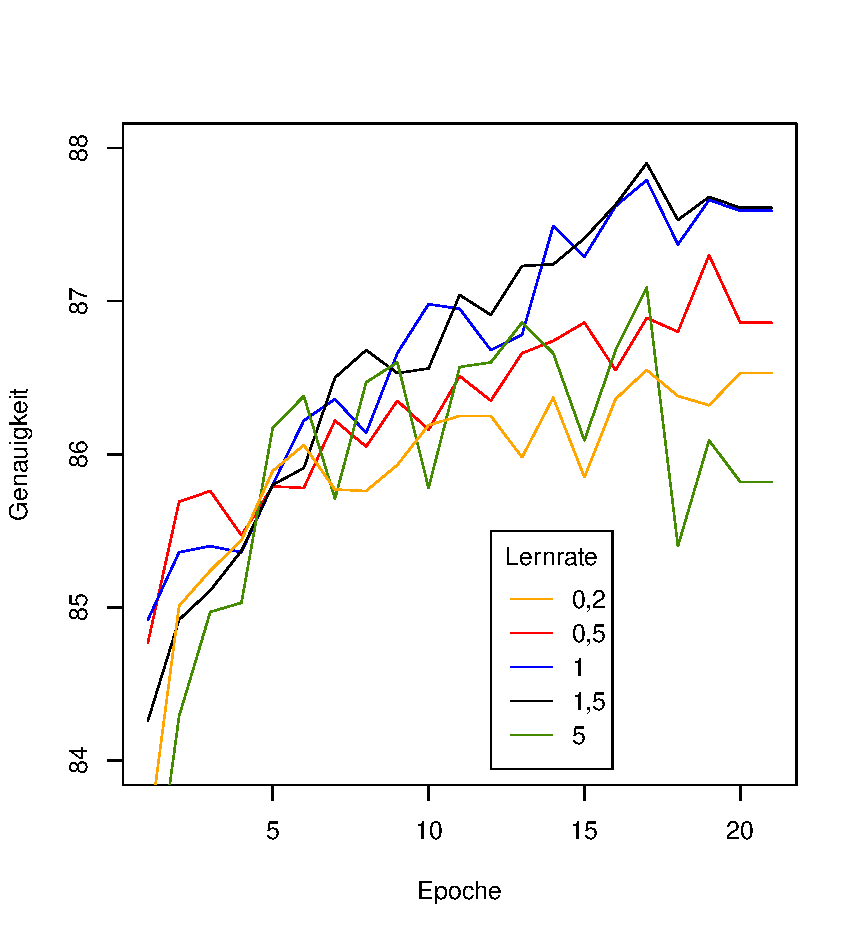
\includegraphics[scale=0.9]{./bilder/learningrate}
	\caption{Training mit verschiedenen Lernraten}
	\label{fig:learningrate}
\end{figure}
Zur Ermittlung der optimalen Lernrate haben wir unser Netzwerk für 20 Epochen mit verschiedenen Lernraten trainieren lassen. In Abbildung \ref{fig:learningrate} sind die Ergebnisse mit einer Messung der Genauigkeit nach jeder Epoche dargestellt. Bei einer Lernrate von 5 ist deutlich das \textit{overfitting} ab Generation 17 zu erkennen. Hier werden zu starke Anpassungen vorgenommen, weshalb sich die Genauigkeit vom Optimum entfernt. Lernraten unter Eins hingegen nähern sich dem Optimum erst gar nicht genug an. Die Lernraten 1 und $1,5$ liefern hier die besten Ergebnisse. Da das Training mit einer Rate von $1,5$ weniger große Ausschläge zeigt, wurde sich für diese Lernrate entschieden.
\section{Batchgröße}
\begin{figure}[H]
	\centering
	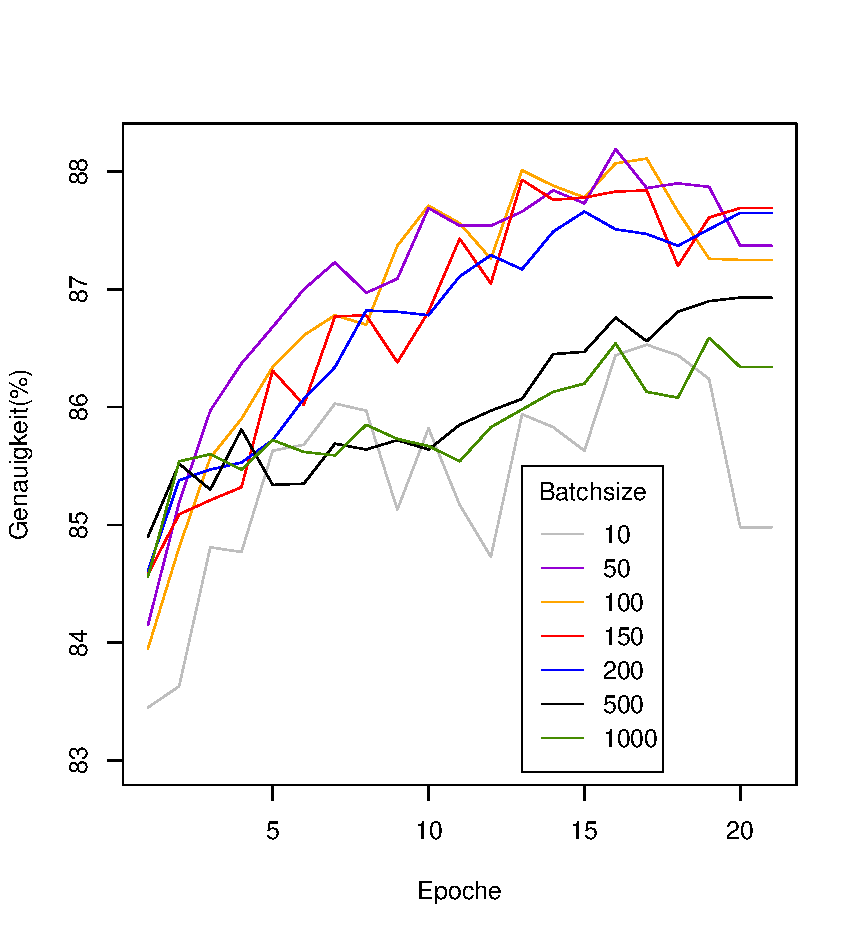
\includegraphics[scale=0.9]{./bilder/batchsize_measurement}
	\caption{Training mit verschiedenen Batchgrößen}
	\label{fig:batchsize}
\end{figure}
